\documentclass[times, utf8, seminar]{fit}

\usepackage{listings}
\usepackage{longtable}
\usepackage{xcolor}
\usepackage{float}
\usepackage{enumitem}
\usepackage{hyperref}
\usepackage{enumerate}
\usepackage{graphicx}
\usepackage{etoolbox}
\usepackage{datetime}
\usepackage{needspace}
\usepackage[compact]{titlesec}
\usepackage{setspace}
\onehalfspacing

\usepackage[parfill]{parskip}

\begin{document}
\widowpenalty=300
\clubpenalty=300

\lstset{
  language=bash,
  backgroundcolor=\color{gray!25},
  basicstyle=\ttfamily \footnotesize,
  breaklines=true,
  prebreak=\raisebox{0ex}[0ex][0ex] {\ensuremath{\hookleftarrow}},
  columns=fullflexible,
  keywords={},
  mathescape=false
}

\title{Agilni \emph{software development},\newline \emph{Continous Integration (CI)}}

\author{Ernad Husremović}
\brindex{DL 2792}
\verzija {0.1.0}

\mentor{mr. Adil Joldić}

\maketitle

\tableofcontents

%\listoftables
%\listoffigures
\newpage

\begin{abstract}

U ovom radu se na bazi konkretnog primjera\footnote{"HOWTO" stil} prezentuje infrastruktura za kontinuiranu integraciju (CI) 

CI infrastruktura je usko vezana za testnu i SCM\footnote{Source Code management} infrastrukturu\citep{agilegit}

Unutar materijala ćemo obraditi implementaciju \href{http://travis-ci.org}{\color{blue}{''Travis Continous Integration''}} za projekat \href{http://redmine.bring.out.ba/projects/knowhow}{\color{blue}{''F18 knowhow''}}.

Za realizaciju ćemo koristiti sljedeće komponente:
\begin{itemize}
  \item Github servis, F18 knowhowERP repozitorij - \url{https://github.com/knowhow/F18\_knowhow}
  \item Travis CI  \url{https://travis-ci.org}
  \item Vagrant test environment  \url{http://vagrantup.com}
\end{itemize}

\keywords{open source software, OSS, travis, CI, continuous integration, vagrant, github, git}
\end{abstract}

% abstract end

\begin{document}
\chapter{Uvod}

\section{Zašto ''Continuous integration'' ?}

Mnogi softverski projekti imaju skriveno kašnjenje između trenutka kada developerski tim kaže "Gotovi smo" i stvarnog trenutka kada je softwarew spreman za isporuku klijentu\citep[str. 183]{agileart}. Nekada je se to kašnjenje može rastegnuti na mjesece.
Spajanje pojedinih komponenti, kreiranje ''installer''-a, kreiranje inicijalne verzije baze podatataka, kreiranje korisničkog uputstva, itd.
U međuvremenu, kompletan tim je pod stresom, ne uzimajući u obzir činjenicu da će ove "post-development" procedure trajati tako dugo. Takvo stanje redovno generira dodatne greške i kašnjenje.
Kontinuirana integracija (CI) prevenira ovakve situacije. Ona obezbjeđuje da se nakon svakog novog commit-a kreira i testira nova verzija software-a. CI omogućava da se odmah nakon razvojnog ciklusa korisniku može isporučiti nova verzija (produkcija).

\begin{quotation}
\noindent \emph{\large Glavni cilj CI-a je mogućnost isporuke (eng. deployment) projekta korisniku u svako vrijeme.}
\end{quotation}

\section{Travis CI}
''Travis CI'' je slobdan CI sistem za opensource developere. Jedini preduslov je da se sofverski repozitorij koji ''travis'' pokriva nalazi na ''github''-u.

Travis funkcioniše tako što se aktivacijom usluge za određenih github projekat, nakon svakog ''commit''-a keira vagrant box\footnote{Više o vagrantu materijalu ''Agilni software development, test \& deploy''\citep[str. 3]{agiletestdeploy}}. Po kreiranju vagrant box-a, pokreću se komande i vrši konfiguracija box-a u skladu sa konfiguracijskim fajlom \href{https://github.com/knowhow/F18_knowhow/blob/master/.travis.yml}{\color{blue}{.travis.yml}}.

Interesatno je uočiti da je kompletan projekat spoznoriran od više sofverskih vendora koji na principu sponzorstva dodjeljuju dio svoje infrastrukture projektu\footnote{Organizacija projekta je u potpunosti u duhu ''opensource''-a, nema šta.}


\begin{figure}[H]
\centering
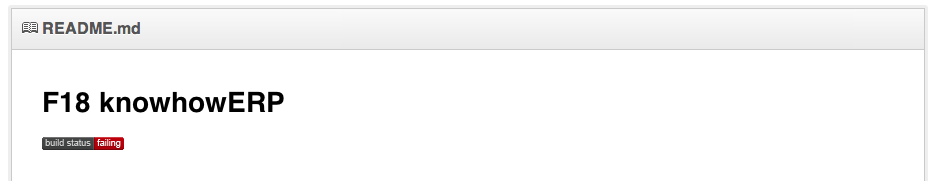
\includegraphics[width=15cm]{img/F18_failing.png}
\caption{travis F18\_knowhowERP build neuspješan - ''failing - red build''}
\end{figure}

\begin{figure}[H]
\centering
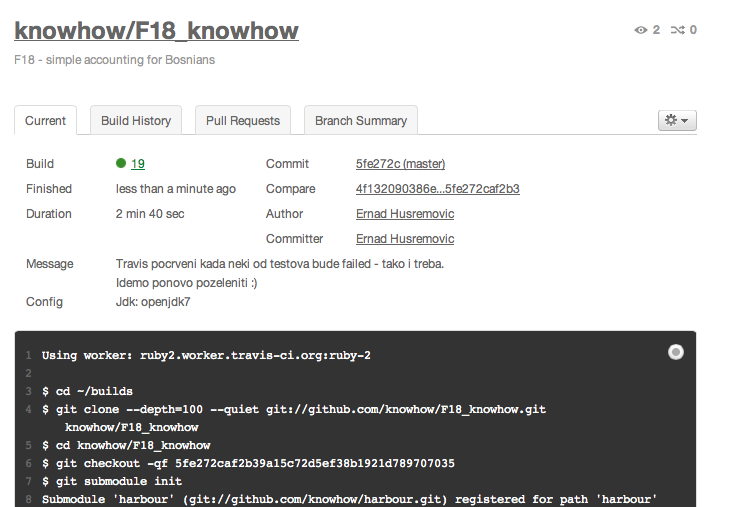
\includegraphics[width=15cm]{img/prvi_green_f18.png}
\caption{travis F18\_knowhowERP prvi uspješan build - ''green build''}
\end{figure}

\begin{figure}[H]
\centering
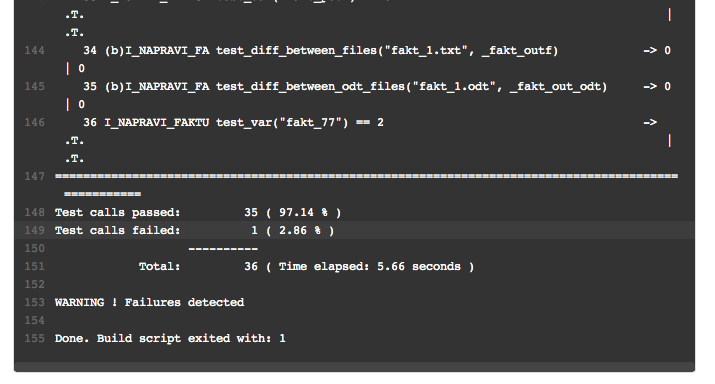
\includegraphics[width=15cm]{img/travis_test_report_failed.png}
\caption{travis F18\_knowhowERP test report - jedan test neuspješan - ''red build''}
\end{figure}


\begin{figure}[H]
\centering
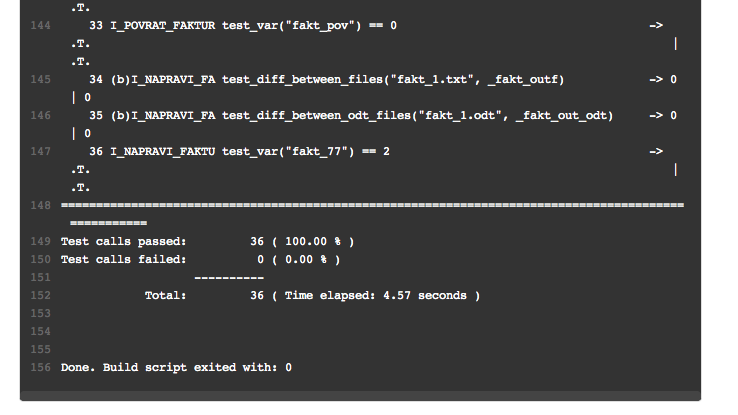
\includegraphics[width=15cm]{img/travis_test_report.png}
\caption{travis F18\_knowhowERP test report prvog uspješnog build-a}
\end{figure}


\begin{figure}[H]
\centering
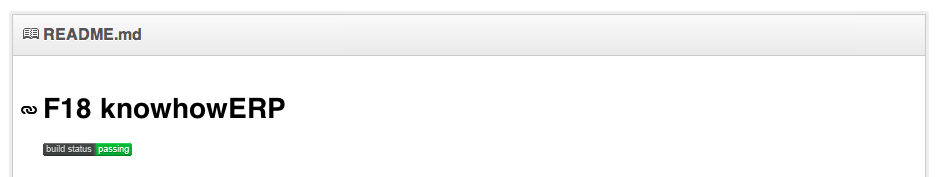
\includegraphics[width=15cm]{img/F18_green.png}
\caption{travis F18\_knowhowERP uspješno - ''green''}
\end{figure}


\begin{figure}[H]
\centering
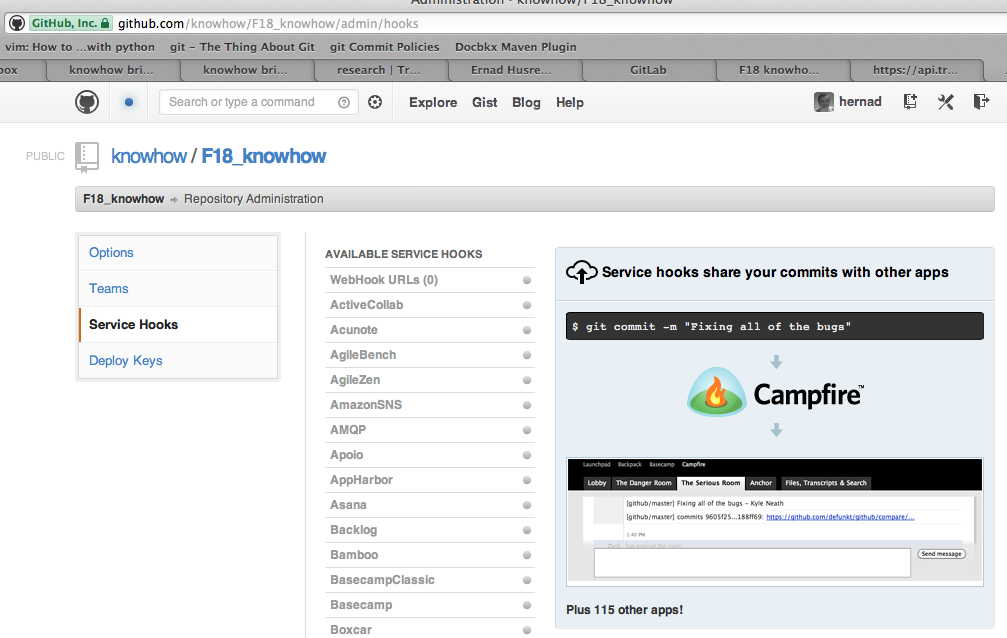
\includegraphics[width=15cm]{img/github_webhook_1.png}
\caption{github travis ''webhook''}
\end{figure}

\begin{figure}[H]
\centering

\includegraphics[width=7cm]{img/github_webhook_2.png}
\caption{github travis ''webhook'' /2}
\end{figure}

\begin{figure}[H]
\centering
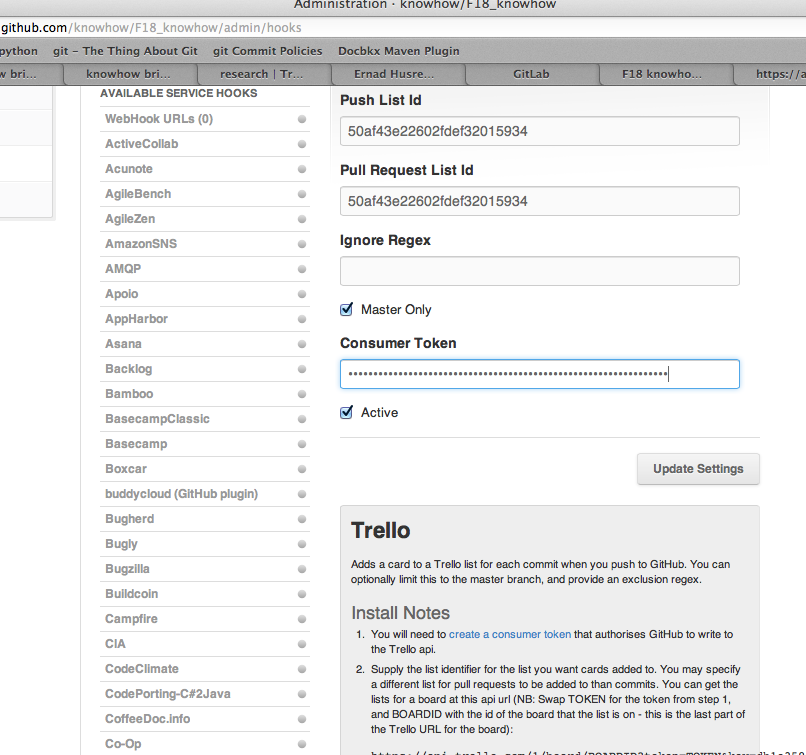
\includegraphics[width=15cm]{img/github_webhook_trello_1.png}
\caption{github trello ''webhook'' /1}
\end{figure}


\begin{figure}[H]
\centering
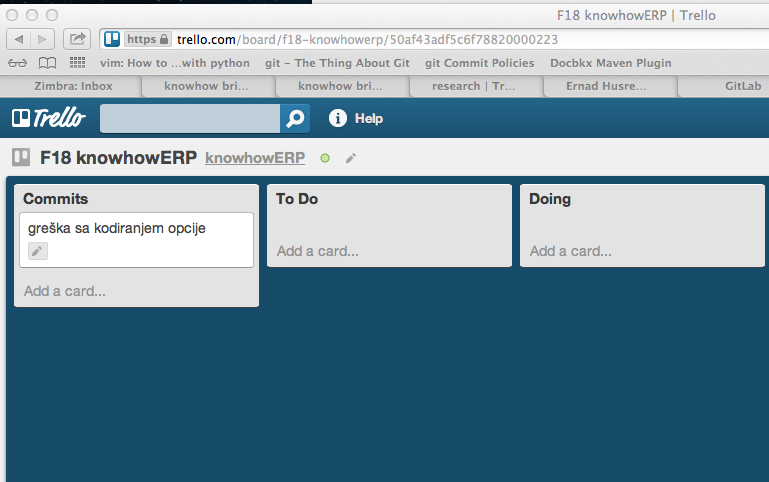
\includegraphics[width=15cm]{img/github_webhook_trello_2.png}
\caption{Prikaz ''commit''-a na trello listi ''Commmits''}
\end{figure}


\begin{figure}[H]
\centering
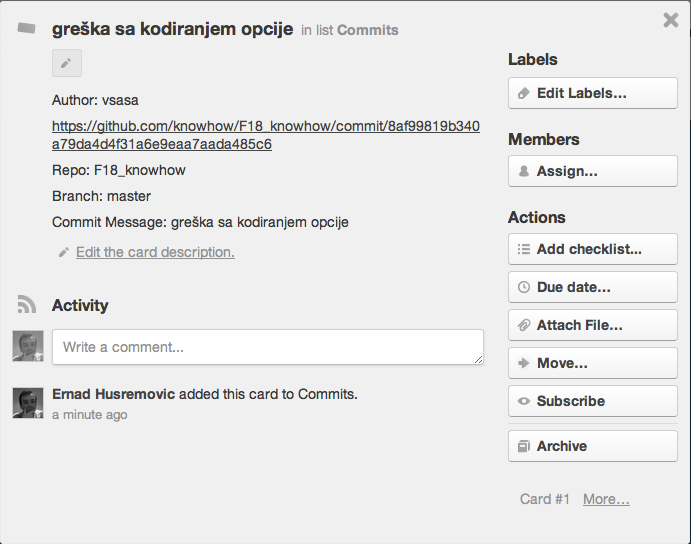
\includegraphics[width=12cm]{img/github_webhook_trello_3.png}
\caption{Git ''commit'' kao ''trello card''}
\end{figure}



\begin{figure}[H]
\centering
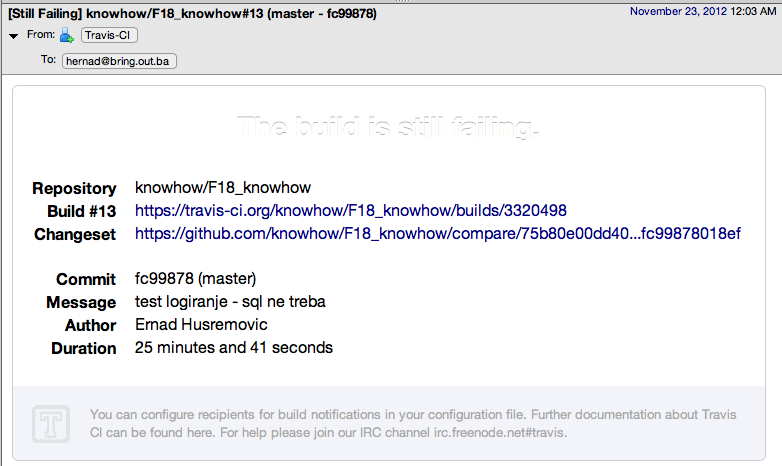
\includegraphics[width=12cm]{img/travis_email_notification.png}
\caption{Travis email notifikacija}
\end{figure}




\bibliography{literatura}
\bibliographystyle{fit}

\appendix


\end{document}
